\documentclass{standalone}
\usepackage{tikz}
\usetikzlibrary{patterns, positioning}


\begin{document}
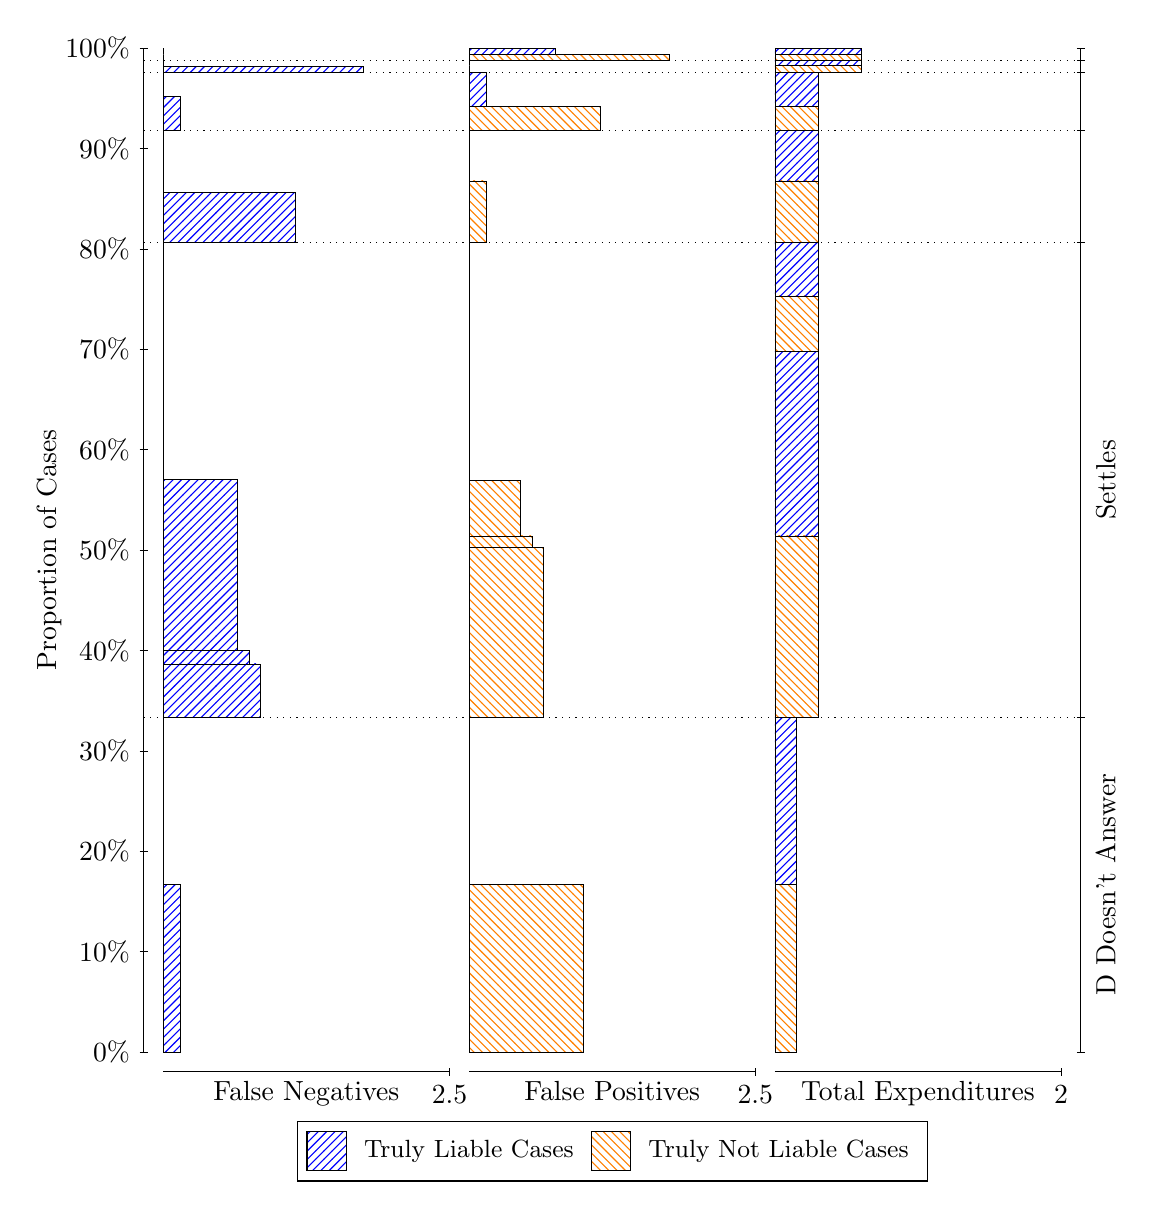
\begin{tikzpicture}
\draw[black, very thin] (1.5,1.75) -- (1.5,14.5);
\node[rotate=90, text=black, anchor=center] at (0.3, 8.125) {Proportion of Cases};
\draw[black, very thin] (1.45,1.75) -- (1.55,1.75);
\node[text=black, anchor=east] at (1.45, 1.75) {0\%};
\draw[black, very thin] (1.45,3.025) -- (1.55,3.025);
\node[text=black, anchor=east] at (1.45, 3.025) {10\%};
\draw[black, very thin] (1.45,4.3) -- (1.55,4.3);
\node[text=black, anchor=east] at (1.45, 4.3) {20\%};
\draw[black, very thin] (1.45,5.575) -- (1.55,5.575);
\node[text=black, anchor=east] at (1.45, 5.575) {30\%};
\draw[black, very thin] (1.45,6.85) -- (1.55,6.85);
\node[text=black, anchor=east] at (1.45, 6.85) {40\%};
\draw[black, very thin] (1.45,8.125) -- (1.55,8.125);
\node[text=black, anchor=east] at (1.45, 8.125) {50\%};
\draw[black, very thin] (1.45,9.4) -- (1.55,9.4);
\node[text=black, anchor=east] at (1.45, 9.4) {60\%};
\draw[black, very thin] (1.45,10.675) -- (1.55,10.675);
\node[text=black, anchor=east] at (1.45, 10.675) {70\%};
\draw[black, very thin] (1.45,11.95) -- (1.55,11.95);
\node[text=black, anchor=east] at (1.45, 11.95) {80\%};
\draw[black, very thin] (1.45,13.225) -- (1.55,13.225);
\node[text=black, anchor=east] at (1.45, 13.225) {90\%};
\draw[black, very thin] (1.45,14.5) -- (1.55,14.5);
\node[text=black, anchor=east] at (1.45, 14.5) {100\%};

\draw[black, very thin] (13.4,1.75) -- (13.4,14.5);
\draw[black, very thin] (13.35,1.75) -- (13.45,1.75);
\node[anchor=west] at (13.35, 1.75) {};
\draw[black, very thin] (13.35,6) -- (13.45,6);
\node[anchor=west] at (13.35, 6) {};
\draw[black, very thin] (13.35,12.03) -- (13.45,12.03);
\node[anchor=west] at (13.35, 12.03) {};
\draw[black, very thin] (13.35,13.453) -- (13.45,13.453);
\node[anchor=west] at (13.35, 13.453) {};
\draw[black, very thin] (13.35,14.194) -- (13.45,14.194);
\node[anchor=west] at (13.35, 14.194) {};
\draw[black, very thin] (13.35,14.347) -- (13.45,14.347);
\node[anchor=west] at (13.35, 14.347) {};
\draw[black, very thin] (13.35,14.5) -- (13.45,14.5);
\node[anchor=west] at (13.35, 14.5) {};

\draw[black, very thin, pattern color=blue, pattern=north east lines] (1.75,1.75) rectangle (1.968,3.875);
\draw[black, very thin, pattern color=orange, pattern=north west lines] (1.75,3.875) rectangle (1.75,6);
\draw[black, very thin, pattern color=blue, pattern=north east lines] (1.75,6) rectangle (2.9853,6.678);
\draw[black, very thin, pattern color=blue, pattern=north east lines] (1.75,6.678) rectangle (2.84,6.8462);
\draw[black, very thin, pattern color=blue, pattern=north east lines] (1.75,6.8462) rectangle (2.6947,9.0223);
\draw[black, very thin, pattern color=orange, pattern=north west lines] (1.75,9.0223) rectangle (1.75,12.03);
\draw[black, very thin, pattern color=blue, pattern=north east lines] (1.75,12.03) rectangle (3.4213,12.669);
\draw[black, very thin, pattern color=orange, pattern=north west lines] (1.75,12.669) rectangle (1.75,13.453);
\draw[black, very thin, pattern color=blue, pattern=north east lines] (1.75,13.453) rectangle (1.968,13.885);
\draw[black, very thin, pattern color=orange, pattern=north west lines] (1.75,13.885) rectangle (1.75,14.194);
\draw[black, very thin, pattern color=blue, pattern=north east lines] (1.75,14.194) rectangle (4.2933,14.266);
\draw[black, very thin, pattern color=orange, pattern=north west lines] (1.75,14.266) rectangle (1.75,14.347);
\draw[black, very thin, pattern color=orange, pattern=north west lines] (1.75,14.347) rectangle (1.75,14.415);
\draw[black, very thin, pattern color=blue, pattern=north east lines] (1.75,14.415) rectangle (1.75,14.5);
\draw[black, very thin, pattern color=orange, pattern=north west lines] (5.6333,1.75) rectangle (7.0867,3.875);
\draw[black, very thin, pattern color=blue, pattern=north east lines] (5.6333,3.875) rectangle (5.6333,6);
\draw[black, very thin, pattern color=orange, pattern=north west lines] (5.6333,6) rectangle (6.578,8.1593);
\draw[black, very thin, pattern color=orange, pattern=north west lines] (5.6333,8.1593) rectangle (6.4327,8.3042);
\draw[black, very thin, pattern color=orange, pattern=north west lines] (5.6333,8.3042) rectangle (6.2873,9.0077);
\draw[black, very thin, pattern color=blue, pattern=north east lines] (5.6333,9.0077) rectangle (5.6333,12.03);
\draw[black, very thin, pattern color=orange, pattern=north west lines] (5.6333,12.03) rectangle (5.8513,12.814);
\draw[black, very thin, pattern color=blue, pattern=north east lines] (5.6333,12.814) rectangle (5.6333,13.453);
\draw[black, very thin, pattern color=orange, pattern=north west lines] (5.6333,13.453) rectangle (7.3047,13.763);
\draw[black, very thin, pattern color=blue, pattern=north east lines] (5.6333,13.763) rectangle (5.8513,14.194);
\draw[black, very thin, pattern color=orange, pattern=north west lines] (5.6333,14.194) rectangle (5.6333,14.275);
\draw[black, very thin, pattern color=blue, pattern=north east lines] (5.6333,14.275) rectangle (5.6333,14.347);
\draw[black, very thin, pattern color=orange, pattern=north west lines] (5.6333,14.347) rectangle (8.1767,14.415);
\draw[black, very thin, pattern color=blue, pattern=north east lines] (5.6333,14.415) rectangle (6.7233,14.5);
\draw[black, very thin, pattern color=orange, pattern=north west lines] (9.5167,1.75) rectangle (9.7892,3.875);
\draw[black, very thin, pattern color=blue, pattern=north east lines] (9.5167,3.875) rectangle (9.7892,6);
\draw[black, very thin, pattern color=orange, pattern=north west lines] (9.5167,6) rectangle (10.062,8.3042);
\draw[black, very thin, pattern color=blue, pattern=north east lines] (9.5167,8.3042) rectangle (10.062,10.649);
\draw[black, very thin, pattern color=orange, pattern=north west lines] (9.5167,10.649) rectangle (10.062,11.352);
\draw[black, very thin, pattern color=blue, pattern=north east lines] (9.5167,11.352) rectangle (10.062,12.03);
\draw[black, very thin, pattern color=orange, pattern=north west lines] (9.5167,12.03) rectangle (10.062,12.814);
\draw[black, very thin, pattern color=blue, pattern=north east lines] (9.5167,12.814) rectangle (10.062,13.453);
\draw[black, very thin, pattern color=orange, pattern=north west lines] (9.5167,13.453) rectangle (10.062,13.763);
\draw[black, very thin, pattern color=blue, pattern=north east lines] (9.5167,13.763) rectangle (10.062,14.194);
\draw[black, very thin, pattern color=orange, pattern=north west lines] (9.5167,14.194) rectangle (10.607,14.275);
\draw[black, very thin, pattern color=blue, pattern=north east lines] (9.5167,14.275) rectangle (10.607,14.347);
\draw[black, very thin, pattern color=orange, pattern=north west lines] (9.5167,14.347) rectangle (10.607,14.415);
\draw[black, very thin, pattern color=blue, pattern=north east lines] (9.5167,14.415) rectangle (10.607,14.5);
\draw[black, dotted] (1.5,6) -- (13.4,6);
\draw[black, dotted] (1.5,12.03) -- (13.4,12.03);
\draw[black, dotted] (1.5,13.453) -- (13.4,13.453);
\draw[black, dotted] (1.5,14.194) -- (13.4,14.194);
\draw[black, dotted] (1.5,14.347) -- (13.4,14.347);
\draw[black, very thin] (1.75,1.5) -- (5.3833,1.5);
\node[text=black, anchor=north] at (3.5667, 1.5) {False Negatives};
\draw[black, very thin] (5.3833,1.45) -- (5.3833,1.55);
\node[text=black, anchor=north] at (5.3833, 1.45) {2.5};

\draw[black, very thin] (5.6333,1.5) -- (9.2667,1.5);
\node[text=black, anchor=north] at (7.45, 1.5) {False Positives};
\draw[black, very thin] (9.2667,1.45) -- (9.2667,1.55);
\node[text=black, anchor=north] at (9.2667, 1.45) {2.5};

\draw[black, very thin] (9.5167,1.5) -- (13.15,1.5);
\node[text=black, anchor=north] at (11.333, 1.5) {Total Expenditures};
\draw[black, very thin] (13.15,1.45) -- (13.15,1.55);
\node[text=black, anchor=north] at (13.15, 1.45) {2};

\node[text=black, centered, rotate=90] at (13.72, 3.875) {D Doesn't Answer};
\node[text=black, centered, rotate=90] at (13.72, 9.015) {Settles};





\draw (7.449999999999999,1.5) node[draw=none] (baseCoordinate) {};
\begin{scope}[align=center]
        \matrix[scale=0.5, draw=black, below=0.5cm of baseCoordinate, nodes={draw}, column sep=0.1cm]{
            \node[rectangle, draw, minimum width=0.5cm, minimum height=0.5cm, pattern color=blue, pattern=north east lines] {}; &
            \node[draw=none, font=\small, text=black] (B) {Truly Liable Cases}; &
            \node[rectangle, draw, minimum width=0.5cm, minimum height=0.5cm, pattern color=orange, pattern=north west lines] {}; &
            \node[draw=none, font=\small, text=black] (B) {Truly Not Liable Cases}; \\
            };
\end{scope}

\end{tikzpicture}
\end{document}